%:
% !TEX TS-program = pdflatex
% !TEX encoding = UTF-8 Unicode

% This is a simple template for a LaTeX document using the "article" class.
% See "book", "report", "letter" for other types of document.

\documentclass{report}
%\documentclass{scrartcl}
%\documentclass[11pt]{report} % use larger type; default would be 10pt
%\setkomafont{disposition}{\normalfont\bfseries}	

\usepackage[utf8]{inputenc} % set input encoding (not needed with XeLaTeX)

%%% PAGE DIMENSIONS
\usepackage{geometry} % to change the page dimensions
\usepackage{amsmath}
\geometry{a4paper} % or letterpaper (US) or a5paper or....
% \geometry{margin=2in} % for example, change the margins to 2 inches all round
% \geometry{landscape} % set up the page for landscape
%   read geometry.pdf for detailed page layout information

\usepackage{booktabs}% http://ctan.org/pkg/booktabs

\usepackage{graphicx} % support the \includegraphics command and options
\usepackage{natbib} % support the \includegraphics command and options
\usepackage{xcolor,colortbl}

\usepackage{multicol}

% \usepackage[parfill]{parskip} % Activate to begin paragraphs with an empty line rather than an indent

%%% PACKAGES
\usepackage{booktabs} % for much better looking tables
\usepackage{array} % for better arrays (eg matrices) in maths
\usepackage{paralist} % very flexible & customisable lists (eg. enumerate/itemize, etc.)
\usepackage{verbatim} % adds environment for commenting out blocks of text & for better verbatim
\usepackage{subfigure} % make it possible to include more than one captioned figure/table in a single float
% These packages are all incorporated in the memoir class to one degree or another...

%%% HEADERS & FOOTERS
\usepackage{fancyhdr} % This should be set AFTER setting up the page geometry
\pagestyle{fancy} % options: empty , plain , fancy
\renewcommand{\headrulewidth}{0pt} % customise the layout...
\lhead{}\chead{}\rhead{}
\lfoot{}\cfoot{\thepage}\rfoot{}

%%% SECTION TITLE APPEARANCE
\usepackage{sectsty}
\allsectionsfont{\sffamily\mdseries\upshape} % (See the fntguide.pdf for font help)
% (This matches ConTeXt defaults)

%%% ToC (table of contents) APPEARANCE
\usepackage[nottoc,notlof,notlot]{tocbibind} % Put the bibliography in the ToC
\usepackage[titles,subfigure]{tocloft} % Alter the style of the Table of Contents
\renewcommand{\cftsecfont}{\rmfamily\mdseries\upshape}
\renewcommand{\cftsecpagefont}{\rmfamily\mdseries\upshape} % No bold!

\usepackage{titling}
\usepackage[brazil]{babel}
\usepackage{xspace}

\usepackage{framed}

\usepackage{setspace}
\onehalfspacing

\usepackage{url}

%\DeclareUnicodeCharacter{00A0}{ }

%%% END Article customizations

%%% The "real" document content comes below...

\begin{document}

\pagestyle{empty} % Removes page numbers

\newcommand{\sw}{\textit{software}\xspace}
\newcommand{\Sw}{\textit{Software}\xspace}
\newcommand{\sws}{\textit{softwares}\xspace}
\newcommand{\iso}{ISO 29110\xspace}
\newcommand{\dsw}{Desenvolvimento de \Sw}

\newcommand{\gp}{Gerente de Projeto\xspace}
\newcommand{\kick}{reunião de \textit{kick-off} do projeto\xspace}
\newcommand{\Kick}{Reunião de \textit{kick-off} do projeto\xspace}
\newcommand{\stake}{\textit{stakeholders}\xspace}
\newcommand{\bline}{\textit{baseline}\xspace}

\newcommand{\amb}{Fatores ambientais da empresa\xspace}
\newcommand{\ativ}{Ativos de processos organizacionais\xspace}

% nomenclaturas de documentação
\newcommand{\planproj}{Plano de Gerenciamento do Projeto\xspace}
\newcommand{\planesc}{Plano de Gerenciamento do Escopo\xspace}
\newcommand{\plancron}{Plano de Gerenciamento do Cronograma\xspace}
\newcommand{\plancusto}{Plano de Gerenciamento de Custos\xspace}
\newcommand{\planqual}{Plano de Gerenciamento da Qualidade\xspace}
\newcommand{\planpess}{Plano de Gerenciamento de Pessoal\xspace}
\newcommand{\plancom}{Plano de Gerenciamento das Comunicações\xspace}
\newcommand{\planrisco}{Plano de Gerenciamento de Riscos\xspace}
\newcommand{\planaq}{Plano de Gerenciamento de Aquisições\xspace}

\newcommand{\termo}{Termo de Abertura do Projeto\xspace}

\newcommand{\bok}{Guia PMBOK$^{\small{\textregistered}}$\xspace}

\newcommand{\pmi}{PMI$^{\small{\textregistered}}$\xspace}

\newcommand{\msp}{Project\xspace}

% schedule forecast
\newcommand{\schfor}{Previsão de cronograma\xspace}
\newcommand{\costfor}{Previsão de custos\xspace}

%\renewcommand{\chapter}{\section}

\newcommand*{\plogo}{\fbox{$\mathcal{PL}$}} % Generic publisher logo

%----------------------------------------------------------------------------------------
%	TITLE PAGE
%----------------------------------------------------------------------------------------

\newcommand*{\titleGP}{\begingroup % Create the command for including the title page in the document
	\centering % Center all text
	\vspace*{\baselineskip} % White space at the top of the page
	
	\rule{\textwidth}{1.6pt}\vspace*{-\baselineskip}\vspace*{2pt} % Thick horizontal line
	\rule{\textwidth}{0.4pt}\\[\baselineskip] % Thin horizontal line

{\Huge Apostila de Gestão de Projetos \\[0.5\baselineskip]  ~Gerenciamento das partes interessadas do projeto}\\[0.2\baselineskip] 

%	{\LARGE \\
%		 }\\[0.2\baselineskip] % Title
	
	\rule{\textwidth}{0.4pt}\vspace*{-\baselineskip}\vspace{3.2pt} % Thin horizontal line
	\rule{\textwidth}{1.6pt}\\[\baselineskip] % Thick horizontal line
	
%	\scshape % Small caps
%	A number of fascinating and life-changing templates \\ % Tagline(s) or further description
%	presented  in a clear and useable way \\[\baselineskip] % Tagline(s) or further description
	\bok e \pmi são marcas registradas do Project Management Institute, Inc.\par % Location and year
	
	\vspace*{2\baselineskip} % Whitespace between location/year and editors
	
	Editado por \\[\baselineskip]
	{\Large Gladistone M. Afonso\par} % Editor list
%	{\itshape The University of California \\ Berkeley\par} % Editor affiliation
	
	\vfill % Whitespace between editor names and publisher logo
	
%	\plogo \\[0.3\baselineskip] % Publisher logo
	{\scshape 2015} \\[0.3\baselineskip] % Year published
	{\large Curso de extensão em Gestão de Projetos\\FASE/FMP}\par % Publisher
	
	\endgroup}

%----------------------------------------------------------------------------------------
%	BLANK DOCUMENT
%----------------------------------------------------------------------------------------

%\begin{document} 
	
%	\pagestyle{empty} % Removes page numbers
	
%	\titleGP % This command includes the title page
	
%\end{document}


%\title{Apostila de Gestão de Projetos\\Gerenciamento de Integracao}
%%\title{Area de conhecimento do \bok \citep{pmbok}}.
%\author{Gladistone M. Afonso}
%
%\date{}
%\maketitle
%\newpage

\titleGP % This command includes the title page

\chapter{Objetivos e características}

O gerenciamento das partes interessadas do projeto inclui os processos necessários para identificar as pessoas, grupos ou organizações que podem impactar ou serem impactadas pelo projeto, analisar as suas expectativas e impactos no projeto e desenvolver estratégias apropriadas para efetivamente engajar as partes interessadas nas decisões e execuções do projeto.

Os processos que fazem parte do gerenciamento das partes interessadas, representados na Figura \ref{fig:proc:ger:stakeholders}, podem ser resumidos em:

\begin{description}

	\item[Identificar as partes interessadas:] identificar as pessoas, grupos ou organizações que podem impactar ou serem impactadas por uma decisão, atividade ou resultado do projeto; analisar e documentar informações relavantes sobre seus interesses, envolvimentos, interdependências, influência e potencial impacto no sucesso do projeto.
	
	\item[Planejar o gerenciamento das partes interessadas:] desenvolver estratégias para efetivamente engajar as partes interessadas durante o ciclo de vida do projeto, baseado na análise de suas necessidades, interesses e potenciais impactos no sucesso do projeto.
	
	\item[Gerenciar o engajamento das partes interessadas:] comunicar e interagir com as partes interessadas para atender suas necessidades, solucionar as questões quando ocorrem e fomentar o engajamento nas atividades durante todo o ciclo de vida do projeto.
	
	\item[Controlar o engajamento das partes interessadas:] monitorar os relacionamentos entre as partes interessadas e ajustar as estratégias para engajar as partes interessadas eliminando resistências e aumentando o suporte ao projeto.

\end{description}

\begin{figure}[!h]
	\centering
	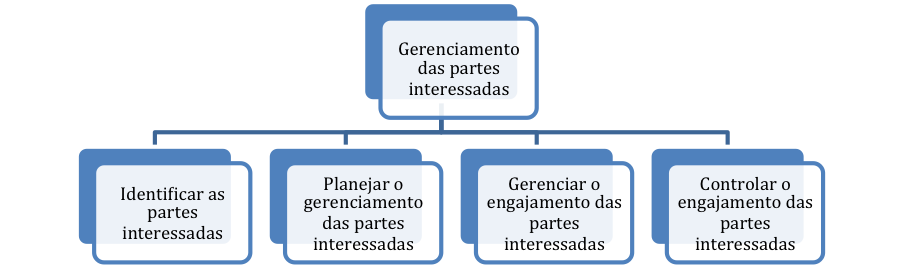
\includegraphics[scale=0.75]{Figuras/gerenciamento_stakeholders.png}
	\caption{Processos do Gerenciamento das partes interessadas}
	\label{fig:proc:ger:stakeholders}
\end{figure}

\chapter{Identificar as partes interessadas}

Processo de identificar as pessoas, grupos ou organizações que podem impactar ou serem impactadas por uma decisão, atividade ou resultado do projeto; analisar e documentar informações relavantes sobre seus interesses, envolvimentos, interdependências, influência e potencial impacto no sucesso do projeto.

O processo de identificar as partes interessadas está representado na Figura \ref{fig:sh:id:efts} e será descrito a seguir.

\begin{figure}[!h]
	\centering
	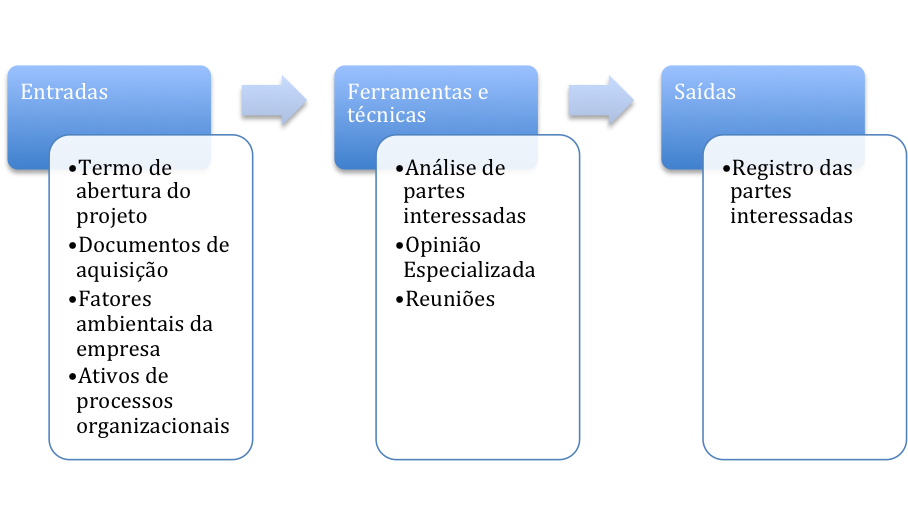
\includegraphics[scale=0.5]{Figuras/stakeholders_efts_identificar.png}
	\caption{Identificar as partes interessadas: entradas, ferramentas, técnicas e saídas}
	\label{fig:sh:id:efts}
\end{figure}

\section{Entradas}

\begin{description}

	\item[Termo de abertura do projeto:] fornece informações sobre partes internas e externas relacionadas com o projeto, tais como: patrocinador, clientes, equipe, grupos, departamentos e outras organizações.
	
	\item[Documentos de aquisição:] as partes dos contratos e os fornecedores são partes interessadas chaves do projeto.
	
	\item[Fatores ambientais da empresa:] cultura e estrutura organizacional, padrões governamentais e da indústria, práticas e hábitos globais ou regionais.
	
	\item[Ativos de processos organizacionais:]	modelos de registro de partes interessadas, lições aprendidas, registros de partes interessadas de projetos anteriores, etc.

\end{description}

\section{Ferramentas e técnicas}

\begin{description}
	
	\item[Análise de partes interessadas:] técnica de sistematicamente juntar e analisar quantitativamente e qualitativamente informações para determinar quais interesses devem ser levados em consideração durante o projeto.
	
	\item[Opinião Especializada:] auxilia na identificação e listagem das partes interessadas.
	
	\item[Reuniões:] podem auxiliar na análise de perfil das partes interessadas.

\end{description}

\section{Saídas}

\begin{description}

	\item[Registro das partes interessadas:] contém informações de identificação, avaliação e classificação das partes interessadas.
	
\end{description}

\chapter{Planejar o gerenciamento das partes interessadas}

Processo de desenvolver estratégias para efetivamente engajar as partes interessadas durante o ciclo de vida do projeto, baseado na análise de suas necessidades, interesses e potenciais impactos no sucesso do projeto.

O processo de planejar o gerenciamento das partes interessadas está representado na Figura \ref{fig:sh:ger:efts} e será descrito a seguir.

\begin{figure}[!h]
	\centering
	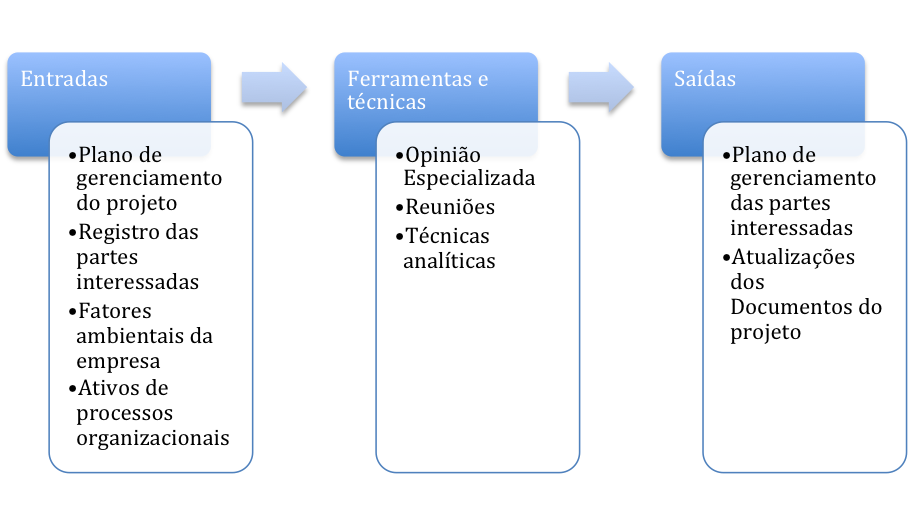
\includegraphics[scale=0.5]{Figuras/stakeholders_efts_gerenciar.png}
	\caption{Planejar o gerenciamento das partes interessadas: entradas, ferramentas, técnicas e saídas}
	\label{fig:sh:ger:efts}
\end{figure}

\section{Entradas}

\begin{description}
	
	\item[Plano de gerenciamento do projeto:] inclui o ciclo de vida selecionado para o projeto e os processos que serão aplicados em cada fase, descrição de como o trabalho será executado para alcançar os objetivos do projeto, descrição de como os requisitos de recursos humanos serão atendidos, descrição de como as mudanças serão controladas, necessidades e técnicas de comunicação entre as partes interessadas, etc.
	
	\item[Registro das partes interessadas:] fornece informações necessárias para planejar as formas de engajar as partes interessadas no projeto.
	
	\item[Fatores ambientais da empresa:] cultura, estrutura, clima e política organizacional, entre outros.
	
	\item[Ativos de processos organizacionais:] lições aprendidas, informações históricas, etc.
	
\end{description}

\section{Ferramentas e técnicas}

\begin{description}
	
	\item[Opinião Especializada:] auxilia na decisão do nível de engajamento necessário a cada estágio do projeto para cada parte interessada.
	
	\item[Reuniões:] utilizadas para determinar o nível de engajamento necessário de todas as partes interessadas.
	
	\item[Técnicas analíticas:] comparação do nível corrente de engajamento com o nível planejado.
		
\end{description}

\section{Saídas}

\begin{description}

	\item[Plano de gerenciamento das partes interessadas:] identifica as estratégias necessárias para efetivamente engajar as partes interessadas.
	
	\item[Atualizações dos Documentos do projeto:] cronograma, registro de partes interessadas, etc.
	
\end{description}

\chapter{Gerenciar o engajamento das partes interessadas}
Processo de comunicar e interagir com as partes interessadas para atender suas necessidades, solucionar as questões quando ocorrem e fomentar o engajamento nas atividades durante todo o ciclo de vida do projeto.

O processo de gerenciar o engajamento das partes interessadas do projeto está representado na Figura \ref{fig:sh:engaja:ger:efts} e será descrito a seguir.

\begin{figure}[!h]
	\centering
	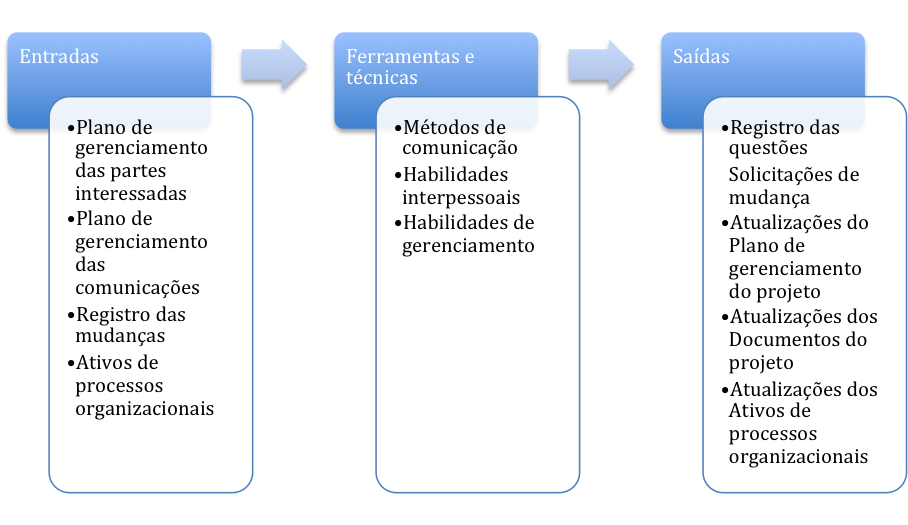
\includegraphics[scale=0.5]{Figuras/stakeholders_efts_ger_engaja.png}
	\caption{Gerenciar o engajamento das partes interessadas: entradas, ferramentas, técnicas e saídas}
	\label{fig:sh:engaja:ger:efts}
\end{figure}

\section{Entradas}

\begin{description}

	\item[Plano de gerenciamento das partes interessadas:] oferece orientações sobre como as várias partes interessadas podem ser melhor envolvidas no projeto.
	
	\item[Plano de gerenciamento das comunicações:] oferece orientações e informações sobre as expectativas das partes interessadas.
	
	\item[Registro das mudanças:] utilizado para documentar as mudanças que ocorrem durante o projeto.
	
	\item[Ativos de processos organizacionais:] requisitos de comunicação organizacional, procedimentos de gerência de questões, procedimentos de controle de mudanças, informações históricas, etc.
	

\end{description}

\section{Ferramentas e técnicas}

\begin{description}
	
	\item[Métodos de comunicação:] identificados para cada parte interessada.
	
	\item[Habilidades interpessoais:] construir confiança, resolver conflitos, escuta ativa, superar resistência à mudança, etc.
	
	\item[Habilidades de gerenciamento:] facilitar consenso em direção aos objetivos do projeto, influenciar pessoas a apoiar o projeto, negociar acordos para satisfazer necessidades do projeto, modificar comportamento organizacional para obter aceite dos resultados do projeto, etc.
	
\end{description}

\section{Saídas}

\begin{description}
	
	\item[Registro das questões:] gerenciar as partes interessadas pode resultar em questões que devem ser registradas.
	
	\item[Solicitações de mudança:] gerenciar as partes interessadas pode resultar em mudanças.
	
	\item[Atualizações do Plano de gerenciamento do projeto:] ocorrem quando requisitos novos ou modificados são identificados.
	
	\item[Atualizações dos Documentos do projeto:] registro de partes interessadas, entre outros.
	
	\item[Atualizações dos Ativos de processos organizacionais:] notificações das partes interessadas, relatórios, apresentações, registros, feedback das partes interessadas, lições aprendidas, etc.
	
\end{description}

\chapter{Controlar o engajamento das partes interessadas}

Processo de monitorar os relacionamentos entre as partes interessadas e ajustar as estratégias para engajar as partes interessadas eliminando resistências e aumentando o suporte ao projeto.

O processo de controlar o engajamento das partes interessadas está representado na Figura \ref{fig:rh:engaja:cont:efts} e será descrito a seguir.

\begin{figure}[!h]
	\centering
	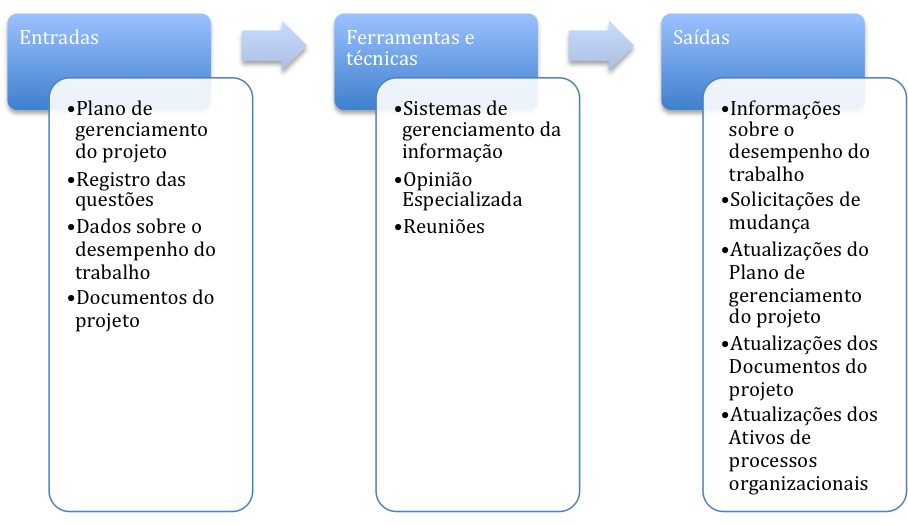
\includegraphics[scale=0.5]{Figuras/stakeholders_efts_cont_engaja.png}
	\caption{Controlar o engajamento das partes interessadas: entradas, ferramentas, técnicas e saídas}
	\label{fig:rh:engaja:cont:efts}
\end{figure}

\section{Entradas}

\begin{description}	

	\item[Plano de gerenciamento do projeto:] inclui o ciclo de vida selecionado para o projeto e os processos que serão aplicados em cada fase, descrição de como o trabalho será executado para alcançar os objetivos do projeto, descrição de como os requisitos de recursos humanos serão atendidos, descrição de como as mudanças serão controladas, necessidades e técnicas de comunicação entre as partes interessadas, etc.
	
	\item[Registro das questões:] atualizado conforme novas questões aparecem e as atuais são resolvidas.
	
	\item[Dados sobre o desempenho do trabalho:] observações e medições identificadas durante a execução das atividades do projeto.
	
	\item[Documentos do projeto:] cronograma, registro de partes interessadas, registro de questões, registro de mudanças, comunicações do projeto, etc.
	
\end{description}

\section{Ferramentas e técnicas}

\begin{description}

	\item[Sistemas de gerenciamento da informação:] capturam, armazenam e distribuem informações para as partes interessadas a respeito de custos, progresso do cronograma e desempenho do projeto.
	
	\item[Opinião Especializada:] garantir identificação e listagem de novas partes interessadas e reavaliação das atuais.
	
	\item[Reuniões:] utilizadas para troca e análise de informações sobre engajamento das partes interessadas.
			
\end{description}

\section{Saídas}

\begin{description}
	
	\item[Informações sobre o desempenho do trabalho:] status das entregas, status de implementação para solicitação de mudanças, etc.
	
	\item[Solicitações de mudança:] análise de desempenho e interação com as partes interessadas geralmente geram solicitações de mudanças.
	
	\item[Atualizações do Plano de gerenciamento do projeto:] plano de gerenciamento de mudanças, plano de gerenciamento de comunicações, plano de gerenciamento de custos, plano de gerenciamento de RH, plano de gerenciamento de qualidade, plano de gerenciamento de requisitos, plano de gerenciamento de riscos, plano de gerenciamento de cronograma, plano de gerenciamento de escopo, plano de gerenciamento de partes interessadas, etc.
	
	\item[Atualizações dos Documentos do projeto:] registro de partes interessadas, registro de questões, etc.
	
	\item[Atualizações dos Ativos de processos organizacionais:] notificações das partes interessadas, relatórios, apresentações, registros, feedback das partes interessadas, lições aprendidas, etc.
	
\end{description}

%\bibliographystyle{plain}
%\bibliographystyle{bibstyle/latex8}     
%\bibliographystyle{apalike-url}     


\bibliographystyle{Bibliografia/apalike-pt}     

%\bibliographystyle{lastchecked}     
            
\bibliography{Bibliografia/research}

\end{document}